\section{Uniform Robustness: Decidability at order four}
\label{section:decidability}
In this section, we prove Theorem \ref{thm:decide}. The techniques naturally apply to lower orders, and we omit their explicit treatment. Recall that we must show how to check the validity of inequality \ref{eq:crux} for all (but finitely many) $n$:
$$
\mathbf{x_n}^T\mathbf{p} \ge r\max_{\mathbf{d}}\mathbf{x_n}^T\mathbf{d} = r ||\mathbf{x_n}|| = r \sqrt{\sum_{j} \sum_{\ell=0}^{m_j-1} \rho_j^n n^{2\ell}}
$$

Our main case distinction is on the number of pairs of complex conjugates among the roots. Thanks to the following old result \cite[Thm. 2]{positive-dominant}, the answer to Ultimate Positivity is trivially NO if there are two pairs of complex conjugates.

\begin{proposition}[Folklore]
\label{prop:folklore}
If the characteristic polynomial has no real root of maximum modulus, then for any initialisation to the sequence, there are infinitely many positive terms, and infinitely many negative terms.
\end{proposition}

On the other hand, if all the roots are real, then again checking the inequality above is trivial: one can simply first check the positivity of the LHS, and then square throughout and use growth arguments, as before. 

Thus, we shall concern ourselves with the case there is one pair of complex conjugate roots. Without loss of generality, we also assume that the real dominant root is $1$.

\subsection{High Level Synopsis}
Ultimate Positivity is a necessary condition for Positivity. Fortunately, it is a a problem that is more amenable to growth arguments. In this subsection, we shall study the exponential polynomial solution, and characterise a set of points in the solution (real exponential polynomial coefficient) space that are guaranteed to result in an Ultimately Positive LRS. The following are major cases we consider:
\begin{align}
\label{eq:unityrep}
u_n &= {\color{red!70!black} z_1 n} + z_0 + \rho^n (x \cos n\theta + y \sin n \theta), ~~ 0< \rho \le 1 \\
\label{eq:fourdom}
u_n &= {\color{red!70!black} z + x\cos n\theta + y\sin n\theta + w(-1)^n} \\
\label{eq:threedom}
u_n &= {\color{red!70!black} z + x\cos n\theta + y\sin n\theta} + w\alpha^n, ~~|\alpha| < 1 \\
\label{eq:twodom}
u_n &= {\color{red!70!black}z + w(-1)^n} + \rho^n(x\cos n\theta + y\sin n\theta), ~~ 0< \rho < 1 \\
\label{eq:onedom}
u_n &= {\color{red!70!black}z} + w\alpha^n + \rho^n(x\cos n\theta + y\sin n\theta), ~~ 0< \rho < 1, |\alpha| < 1
\end{align}

The terms in black become negligibly small relative to the terms in dark red. The cases we draw are based on whether $1$ is a repeated dominant root, or whether there are four, three, two, or one (distinct) dominant roots.

In each of the cases, we have to decide the universal validity of the corresponding version of inequality \ref{eq:crux}. This often entails asking whether some $F(\mathbf{p}, \cos n\theta, \sin n\theta, (-1)^n) \ge G(n)$. The high-level approach is to:
\begin{enumerate}
\item Replace $F(\mathbf{p}, \cos n\theta, \sin n\theta, (-1)^n)$ by $F(\mathbf{p}, \cos \phi, \sin \phi, b)$ (Masser)
\item Argue that $\liminf_n F = \min_{\phi \in [0, 2\pi); b\in\{-1, 1\}} F = \mu$ (Kronecker)
\item Query $\mu$ (First Order Theory of Reals)
\item Give a tighter lower bound on $F(\mathbf{p}, \cos n\theta, \sin n\theta, (-1)^n) - \mu$ than $G$ (Baker) 
\item Based on this, identify an upper bound $N$, beyond which inequality \ref{eq:crux} cannot be violated.
\end{enumerate}

\subsection{Mathematical tools}
\label{arsenal}
Multiplicative dependencies among algebraic numbers can be efficiently elicited. 
 \begin{theorem}[Masser \cite{Masser}]
  \label{thm:abelian}
  Let $e^{i \theta_1},...,e^{i \theta_k}$ be complex algebraic numbers of unit modulus. Consider the free abelian group $L$ defined by $L = \{(\lambda_1, \ldots ,\lambda_k) \in \mathbb{Z}^k: 
  e^{i (\lambda_1 \theta_1 + \cdots +  \lambda_k \theta_k)} = 1 \}$. 
  The group $L$ has a finite generator set $\{ \mathbf{l_1}, \ldots, \mathbf{l_p}\} \subset \mathbb{Z}^k$ with $p \le k$. The generator set can be computed in time polynomial and
  each entry in the generator set is polynomially bounded in the sizes of the representations of $e^{i \theta_1},...,e^{i \theta_k}$.
  \end{theorem}
 Given $e^{2i\theta}$, if an $n$ such that $e^{2i n \theta} = 1$ exists ($\theta$ is a rational multiple of $2\pi$), this $n$ is bounded, and can be efficiently found by enumeration. Similarly, one can check whether $\alpha^n = \beta$ (is $n\theta - \varphi$ ever an integer multiple of $2\pi$?). 
 
 The above owes its potency to the fact that we can use it to abstract the discrete, dense $n\theta$ by the continuous $\phi$. This enabled by Kronecker's theorem on simultaneous Diophantine approximation, as strengthened by \cite{joeljames3, ouaknine2014positivity}
 
 \begin{theorem}[Kronecker \cite{Kronecker}]
  \label{thm:kronecker}
  Let $\theta_1, ... , \theta_k, \phi_1, ... , \phi_k \in [0, 2\pi)$. Then the following are equivalent:
  \begin{enumerate}
\item For every tuple $(\lambda_1,...\lambda_k)$ of integers with 
    $\lambda_1 \theta_1 + \cdots +  \lambda_k \theta_k \in 2\pi\integers$, 
  we have \\$\lambda_1 \phi_1 + \cdots + \lambda_k \phi_k \in 2\pi\integers$.
  \item For any $\epsilon > 0$, there exists an arbitrarily large $n$ such that for all 
    $1 \le j \le k$ we have $| n \theta_j - \phi_j| \le \epsilon$.
    \end{enumerate}
  \end{theorem}
  
This immediately implies that
\begin{equation}
\liminf_{n \in \naturals} F(\mathbf{p}, \cos n\theta, \sin n\theta, (-1)^n) = \min_{\phi \in [0, 2\pi); b\in\{-1, 1\}} F(\mathbf{p}, \cos \phi, \sin \phi, b) = \mu
\end{equation}

We now turn to computing $\mu$. Fortunately, $F$ is multilinear, and, given $\mathbf{p}$, all the constants involved are algebraic. Thus, we can use the First Order Theory of the Reals. Let $\sigma(a_1, a_2, b)$ denote $a_1^2 + a_2^2 = 1 \land b^2 =1$. Then, $\mu$ is the unique satisfying assignment of the following formula $\chi(\mu)$
$$
(\forall a_1, a_2, b.~ \sigma(a_1, a_2, b) \implies F(\mathbf{p}, a_1, a_2, b) \ge \mu) \land (\exists a_1, a_2, b.~ \sigma(a_1, a_2, b) \land F(\mathbf{p}, a_1, a_2, b) = \mu)
$$
Renegar's Theorem (Theorem \ref{thm:renegar}) asserts that this algebraic $\mu$ can be computed via quantifier elimination. Finally, we note that when $\theta$ is not a rational multiple of $2\pi$, the minimum of $1 - \cos(n\theta - \varphi)$ is attained at most once: we can use Theorem \ref{thm:abelian} to check if this is the case. In fact, we can provide a threshold $N_1$ beyond which $n\theta \ne \varphi$. 

We now invoke Baker's theorem to lower bound $[n\theta - \varphi]_{2\pi}$. The statement we present is a sharp formulation due to Baker and W{\"u}stholz \cite{baker}. In the following, $\log z$ refers to the principal branch, i.e. $\log |z| + i \arg z$, where $\arg z \in (-\pi, \pi]$.

\begin{theorem}[Baker]
\label{thm:baker}
Let $\alpha_1, \dots, \alpha_m \in \algebraics$ be different from $0$ and $1$, and let $b_1, \dots, b_m \in \integers$. Write
$$
\Lambda = b_1 \log \alpha_1 + \dots + b_m \log \alpha_m
$$
Let $A_1, \dots, A_m, B \ge e$ be such that for each $j \in [m]$, $A_j$ is an upper bound for the height of $\alpha_j$, and $B$ is an upper bound for $|b_j|$. Let $d$ be the degree of the extension field $\rationals(\alpha_1, \dots, \alpha_m)$ over $\rationals$. If $\Lambda \ne 0$, then
$$
\log |\Lambda| > -(16md)^{2(m+2)}\log A_1 \dots \log A_m \log B
$$  
\end{theorem}

In our context $m=2$ ($m=1$ is even simpler), $\alpha_1 = e^{i\theta}$, and $\alpha_2 = e^{-i\varphi}$, $b_1 = n$, $b_2 = 1$. $A_1, A_2, d$ are all fixed constants, $B = n$. Hence, beyond $M$ for which $[n\theta - \varphi]_{2\pi} \ne 0$,
\begin{equation}
|\Lambda| = [n\theta - \varphi]_{2\pi} > \exp(-(32d)^8 \log A_1 \log A_2 \log n)
\end{equation}
Simplifying, we conclude there exists a polynomial $H$ such that for all $n \ge M$,
\begin{equation}
[n\theta - \varphi]_{2\pi} > \frac{1}{H(n)}
\end{equation}
As argued in \cite{joeljames3} using the Taylor series expansion, we can further claim that there exists an $N$, and another polynomial $g$, such for all $n \ge N$
\begin{equation}
\label{eq:baker}
1 - \cos(n\theta - \varphi) > \frac{1}{g(n)}
\end{equation}

We are now ready resolve each case, in roughly increasing order of non-triviality. 

\subsection{Two distinct dominant roots}
This scenario corresponds to equation \ref{eq:twodom}. Here, the inequality is
\begin{equation}
z + w(-1)^n + \rho^n(x \cos n\theta + y \sin n\theta) \ge r\sqrt{2 + \rho^{2n}}
\end{equation}
This is non-trivial only when the limiting values of both the (minimal) LHS and RHS are equal, \\i.e. $z - |w|= r\sqrt{2}$. Depending on the sign of $w$, we must have have for all (but finitely many) odd (or even) $n$,
\begin{equation}
\rho^n(x \cos n\theta + y \sin n\theta) \ge r\left(\frac{\rho^{2n}}{\sqrt{2 + \rho^{2n}} + \sqrt{2}}\right)
\end{equation}
However, the RHS is always positive, while the LHS will be negative for infinitely many odd (and even!) $n$. Hence, we can return NO.

\subsection{Unity as a repeated dominant root}
In this case (equation \ref{eq:unityrep}), given the centre and $r$, we need to check whether for all (but finitely many) $n$:
\begin{equation}
z_1 n + z_0 + \rho^n (x \cos n\theta + y \sin n \theta) \ge r\sqrt{n^2 + 1 + \rho^{2n}}
\end{equation}
This can trivially be resolved with growth arguments if $z_1 \ne r$, so we will assume $z_1 = r$. Subtracting $rn$ from both sides,

\begin{equation}
z_0 + \rho^n (x \cos n\theta + y \sin n \theta) \ge r\left( \frac{1 + \rho^{2n}}{n+ \sqrt{n^2 + 1 + \rho^{2n}}}\right)
\end{equation}

The RHS decays to $0$ linearly. Thus, the only case that is non-trivial is when $\rho = 1$, $\theta$ is not a rational multiple of $2\pi$, and $z_0^2 = x^2 + y^2$. In this case, our inequality can be written as
\begin{equation}
z_0(1 - \cos(n\theta - \varphi)) \ge r\left( \frac{2}{n+ \sqrt{n^2 + 2}}\right)
\end{equation}

As noted in inequality \ref{eq:quadraticdecay}, the LHS is upper-bounded by $c/n^2$ for infinitely many $n$, while the RHS can be lower bounded by $r/n$. Thus, the above inequality will be violated for infinitely many $n$. We can therefore return NO for $r$-Robust Uniform Ultimate Positivity as well as $r$-Robust Positivity.

\subsection{Four distinct dominant roots}
This corresponds to equation \ref{eq:fourdom}. The relevant inequality is
\begin{equation}
z + x \cos n\theta + y\sin n\theta + w \ge r\sqrt{3}
\end{equation}

We can detect if $\theta$ is a rational multiple of $2\pi$ (Theorem \ref{thm:abelian}), in which case checking the inequality is trivial. Otherwise, we invoke Theorem \ref{thm:kronecker} to argue that it suffices to check the truth of this sentence in First Order Theory of the Reals:
\begin{equation}
\forall q_1, q_2, q_3. \left(q_1^2 + q_2^2 = 1 \land q_3^2 = 1\right) \Rightarrow z + xq_1 + yq_2 + wq_3 - r\sqrt{3} \ge 0
\end{equation}
Of course, the above form doesn't fit the grammar, but $z, x, y, w, r, \sqrt{3}$ are all algebraic constants, and accessible in this theory. The truth of this sentence can be evaluated: in fact, it is equivalent to
\begin{equation}
\label{eq:cone}
z - |w| - \sqrt{x^2 + y^2} - r\sqrt{3} \ge 0
\end{equation}

\subsection{One dominant root}
This corresponds to equation \ref{eq:onedom}. Our critical inequality here is
\begin{equation}
z + w\alpha^n + \rho^n(x \cos n\theta + y \sin n \theta) \ge r\sqrt{1 + \alpha^{2n} + \rho^{2n}}
\end{equation}
As before, we note that this is interesting only when $z = r$, and subtract $r$ from both sides
\begin{equation}
w\alpha^n + \rho^n(x \cos n\theta + y \sin n \theta) \ge r\left(\frac{\alpha^{2n} + \rho^{2n}}{1 + \sqrt{1 + \alpha^{2n} + \rho^{2n}}}\right)
\end{equation}

$\alpha$ must be positive, otherwise the LHS will be negative for infinitely many $n$. Furthermore, $\alpha \ge \rho$ for the same reasons. If $\alpha > \rho$, the problem can again be resolved via growth arguments. We shall therefore assume that $\alpha = \rho$. 
\begin{align}
w + x \cos n\theta + y \sin n \theta &\ge r\left(\frac{2\rho^{n}}{1 + \sqrt{1 + 2\rho^{2n}}}\right)
\end{align}

As before, our problem is non-trivial only if $\theta$ is not a rational multiple of $2\pi$, and $w^2 = x^2 + y^2$. So, we can rearrange as 
\begin{equation}
w(1 - \cos(n\theta - \varphi)) \ge r\left(\frac{2\rho^{n}}{1 + \sqrt{1 + 2\rho^{2n}}}\right)
\end{equation}
We appeal to equation \ref{eq:baker} from Baker: there is an $N \in \naturals$ and polynomial $g$ such that for all $n \ge N$, we have the stronger
\begin{equation}
w(1 - \cos(n\theta - \varphi)) > \frac{1}{g(n)} > r \rho^n >  r\left(\frac{2\rho^{n}}{1 + \sqrt{1 + 2\rho^{2n}}}\right)
\end{equation}
Decidability follows by explicitly checking the original inequality up to $N$.

\subsection{Three distinct dominant roots}
Our final case corresponds to equation \ref{eq:threedom}, and combines techniques from the previous two subsections. The critical inequality is
\begin{equation}
z + x\cos n\theta + y\sin n\theta + w\alpha^n \ge r\sqrt{2 + \alpha^{2n}}
\end{equation}
We first quickly dispose of the case $\theta$ is a rational multiple of $2\pi$. As in the previous cases, the critical scenario is when the minimum of the finitely many values $z + x\cos n\theta + y\sin n\theta $ can take is $r\sqrt{2}$. Let this value be taken when $n = qm + r$. Beyond a sufficient computable threshold, we must therefore have for all $m$
\begin{equation}
w\alpha^{qm+r} \ge r\left(\frac{\alpha^{2(qm+r)}}{\sqrt{2}+ \sqrt{2+\alpha^{2(qm+r)}}}\right)
\end{equation}

Here $\alpha$ is real. If $\alpha > 0$, then this inequality will eventually always be satisfied. If $\alpha < 0$: this inequality is eventually always satisfied if and only if either $w>0$ and $qm+r$ is always even, or $w<0$ and $qm+r$ is always odd. This can easily be checked.

In the remainder of this section, we shall assume that $\theta$ is not a rational multiple of $2\pi$. We use Theorem \ref{thm:kronecker} (Kronecker) to argue $n\theta$ (modulo $2\pi$) is dense in $[0, 2\pi)$. The critical case arises when the inequality can be rearranged as
$$
r\sqrt{2} + q(1 - \cos(n\theta - \varphi)) + w\alpha^n \ge r\sqrt{2 + \alpha^{2n}} \Leftrightarrow q(1 - \cos(n\theta - \varphi)) \ge -w\alpha^n + r\left(\frac{\alpha^{2n}}{\sqrt{2}+\sqrt{2 + \alpha^{2n}}}\right)
$$
As in the previous case, we use equation \ref{eq:baker} due to Baker to argue a lower bound on the LHS that is much tighter than the RHS, that holds from a computable $N$ onwards. We finish off by explicitly checking the original inequality explicitly up to $N$.

\section{Non-uniform Robustness: Decidability at order five}
\label{section:decidability2}
In this section, we redeploy the sophisticated arsenal we invoked in \S\ref{arsenal} to prove Theorem \ref{thm:decide2}. As before, the techniques naturally apply to lower orders, and we omit their explicit treatment. Recall equation \ref{eq:grouping} and the surrounding discussion:
\begin{equation}
u_n/n^d\rho^n = \begin{bmatrix}
{\color{red!70!black} \mathbf{q}_{dom}^T(n) } & \mathbf{q}_{res}^T(n)
\end{bmatrix}
\begin{bmatrix}
{\color{red!70!black} \mathbf{p}_{dom}} \\
\mathbf{p}_{res}
\end{bmatrix}
\end{equation}
The crucial first task is to check whether for all points in the neighbourhood, \\$\liminf_{n\in\naturals}\mathbf{q}_{dom}^T(n)\mathbf{p}_{dom} = \mu \ge 0$. Observe that through Theorems \ref{thm:abelian}, \ref{thm:kronecker}, \ref{thm:renegar} (Masser, Kronecker, and Renegar) we have already discussed the means to check the inequality for a particular $\mathbf{p}$, through the First Order Theory of Reals. Let $\psi(\mathbf{p})$ (resp.\ $\psi_0(\mathbf{p})$) be the quantifier free formula that expresses $\mu > 0$ (resp.\ $\mu = 0$). We simply query the truth of
\begin{equation}
\label{eq:firsttask}
\forall \mathbf{p'}.~||\mathbf{p'} - \mathbf{p}|| \le r \Rightarrow (\psi(\mathbf{p'}) \lor \psi_0(\mathbf{p'}))
\end{equation}
If there are no residual terms, we are already done at this point. In the event residual terms have non-zero contribution, decidability hinges on whether we can handle points where $\mu = 0$. If there are two pairs of complex conjugates among the dominant roots, then all five terms are dominant (recall Proposition \ref{prop:folklore}!)

\begin{figure}[h]

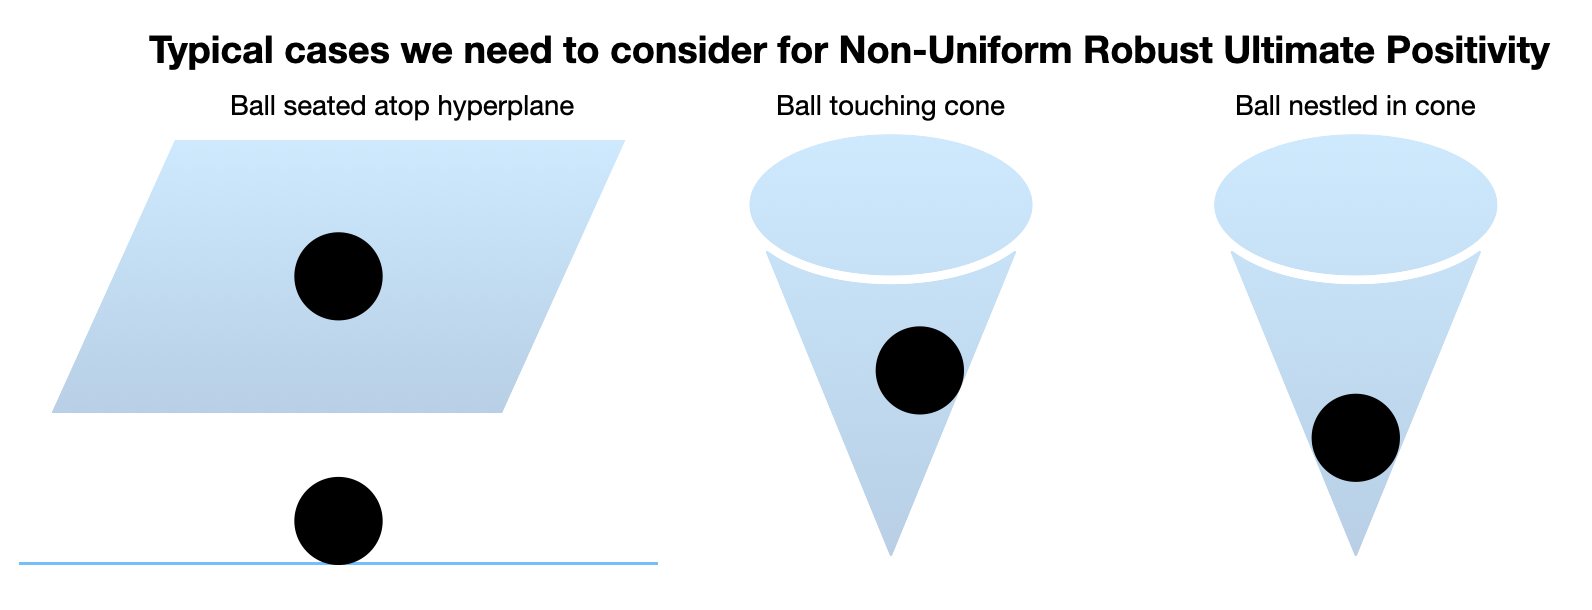
\includegraphics[width=\textwidth]{picture1.png}
\caption{Visual intuition}
\label{fig:geometricpicture}
\end{figure}

Hence, we consider that there is at most one complex conjugate pair among the dominant roots. This requires slightly more insight of the geometrical nature of the solution set of $\psi_0$ (Figure \ref{fig:geometricpicture}). See \cite{originalstacs,originalarxiv} for an exposition of the geometric intuition. If there are just one or two dominant terms, they are necessarily real. The region $\mu(\mathbf{p}) = 0$ will simply be the union of at most two hyperplanes. ($z = 0$, or $z - |w| = 0$). Here, the intersection of the ball with $\mu = 0$ consists of at most two points. Since Ultimate Positivity is decidable up to order $5$ \cite{joeljames3}, it can explicitly be checked.

Finally, let there be one pair of complex conjugates $e^{\pm i\theta}$ among the dominant roots. It is clear that if $\theta$ is a rational multiple of $2\pi$, $\mu = 0$ will be a union of finitely many hyperplanes (of the form $z - |w| - x\cos \theta_0 - y\sin \theta_0 = 0$). Here again, the finite intersection can be explicitly checked. In the case when $e^{i\theta}$ is not a root of unity, we recall equation \ref{eq:cone}: the set of $\mathbf{p}$ for which $\mu = 0$ is given by
\begin{equation}
z - |w| - \sqrt{x^2 + y^2} = 0
\end{equation}
In this case, it is a union of \textit{infinitely} many hyperplanes of the form $z - |w| - x \cos \phi - y\sin \phi = 0$. As established by the validity of equation \ref{eq:firsttask}, the centre of the neighbourhood is distance at least $r$ away from each of these hyperplanes. If the surface of the $r$-ball touches any of these hyperplanes, the point must be obtained by traversing along the normal from the centre. Thus, the point must be $(z_0 - \frac{r}{\sqrt{3}}, w_0 \pm \frac{r}{\sqrt{3}}, x_0 + \frac{r}{\sqrt{3}}\cos\phi, y_0 +  \frac{r}{\sqrt{3}}\sin\phi, v_0)$. Note that the residual coordinate is unchanged! Substituting this into the hyperplane equation gives us a quadratic equation in $\cos \phi$: this holds for zero, one, two, or all $\phi$. We already know how to handle a finite intersection.

If this holds for all $\phi$, then we use Theorem \ref{thm:kronecker} (Kronecker's density) to argue that for every $n$, there exists a point on the surface of the ball such that the dominant contribution is zero. As observed, the residual part is the same as the centre for such points. Thus, in this case, it is entirely up to the residual terms of the centre to guarantee Robust Ultimate Positivity. This is a decidable instance of regular Ultimate Positivity at lower order, and we are done.
